\documentclass[times, utf8, zavrsni]{fer}
\usepackage{booktabs}
\usepackage{tikz}
\usepackage{algorithmic}
\usepackage{algorithm}
\usepackage{listings}
\usepackage{amsthm}
\newtheorem{theorem}{Teorem}[section]
\newtheorem{definition}{Definicija}[section]
\newtheorem{lemma}{Lemma}[section]
\newtheorem{proposition}{Propozicija}[section]

\begin{document}

\thesisnumber{253}

\title{Prebrojavanje razapinjućih stabala grafa}

\author{Dorian Kablar}

\maketitle

% Ispis stranice s napomenom o umetanju izvornika rada. Uklonite naredbu \izvornik ako želite izbaciti tu stranicu.

% Dodavanje zahvale ili prazne stranice. Ako ne želite dodati zahvalu, naredbu ostavite radi prazne stranice.
\zahvala{Zahvaljujem mentorici, izv. prof. dr. sc. Anamari Nakić, na motivaciji i savjetima prilikom pisanja ovog rada.

Zahvaljujem svojim roditeljima, pogotovo majci, koji su me podržavali u svakoj odluci, i koji su uvijek znali kako pomoći, čak i kad nisam bio svjestan da je pomoć potrebna.}

\tableofcontents

\chapter{Uvod}

Teorija grafova široko je područje s brojnim primjenama u stvarnom svijetu. Njen začetak vezan je uz jedan problem iz stvarnog života. Članak iz 1736. u kojem je švicarski matematičar Leonhard Euler predstavio i rješio problem königsbergskih mostova smatra se prvim pisanim djelom o \textit{teoriji grafova}. No, sam pojam grafa je u široku uporabu ušao tek 1936., kada je Dénes Kőnig objavio monografiju \textit{Theory of finite and infinite graphs}\footnote{engleski prijevod njemačkog originala \textit{Theorie der endlichen und unendlichen Graphen.}}.
Ta se godina uzima kao godina osnutka \textit{teorije grafova} kao zasebne matematičke discipline.

\begin{figure}[htb]
	\centering
	\begin{tikzpicture}[node distance={45mm}, main/.style = {draw, circle}] 
		\node[main] (1) {$A$}; 
		\node[main] (2) [above left of=1] {$B$};
		\node[main] (3) [below left of=1] {$C$};
		\node[main] (4) [right of=1] {$D$};
		\draw (1) -- (2);
		\draw (1)  to [out=175,in=270,looseness=1.5] (2);
		\draw (1) -- (3);
		\draw (1)  to [out=185,in=90,looseness=1.5] (3);
		\draw (1) -- (4);
		\draw (2) -- (4);
		\draw (3) -- (4);
	\end{tikzpicture}
	\caption{Graf koji prikazuje problem königsbergskih mostova.}
\end{figure}

Svoj zamah teorija grafova dobiva tek u drugoj polovici 20. stoljeća, stoga je, s obzirom da je to još uvijek relativno mlada disciplina, puno otvorenih problema koji i danas još uvijek nisu riješeni.

Teorija grafova se primjenjuje u mnogim područjima. U računarskoj znanosti, grafovi su od velikog interesa, s jedne strane kao struktura podataka, a s druge strane zbog algoritama nad grafovima, i raznih drugih primjena. Primjerice, grafovi mogu koristiti u izgradnji \textit{NoSQL} baza podataka, gdje se u čvorove mogu spremati podatci, a u bridove veze između podataka.

U društvenim znanostima, korištenjem softvera za analizu društvenih mreža, teorija grafova se može koristiti, primjerice, za istraživanje širenja neke glasine. U molekularnoj biologiji, grafovi se koriste za modeliranje i analizu molekula/spojeva s kompleksnim međusobnim vezama. Osim navedenih, grafovi imaju svoje primjene i u lingvistici, fizici, kemiji, matematici, i mnogim drugima.

U ovom radu bit će više riječi o podvrsti grafova, \textit{stablima}. Stabla mogu, također, biti od velikog značaja u mnogim granama. Primjerice, recimo da se cestom želi povezati nekoliko gradova. Kako bi izvođači radova što jefitnije te radove obavili, pokušat će naći \textit{minimalno razapinjuće stablo} grafa koji će predstavljati te gradove i udaljenosti između njih. O ovom, i sličnim problemima, bit će više riječi u kasnijim poglavljima ovog rada.

U prvom dijelu iznesene su glavne definicije i rezultati vezani uz grafove i stabla. U drugom dijelu će biti govora o razapinjućim stablima. Prikazani su osnovni rezultati te primjeri računanja broja razapinjućih stabala za familije grafova. 
U trećem iskazan je i dokazan matrični teorem o stablima.
U četvrtom su iskorišteni predstavljeni rezultati za prebrajanje razapinjućih stabala poznatih familija grafova. U petom dijelu je opisan rad aplikacije \textit{Graphelite} za računanje razapinjućih stabala zadanog grafa.

\chapter{Osnovne definicije i rezultati}

Za početak predstavljamo pojam grafa.

\begin{definition}
	\textbf{Jednostavni graf} G sastoji se od nepraznog konačnog skupa $V(G)$, čije elemente zovemo \textbf{vrhovi} grafa G i konačnog skupa $E(G)$ različitih dvočlanih podskupova skupa $V(G)$ koje zovemo \textbf{bridovi}.
\end{definition}

\begin{figure}[htb]
	\centering
	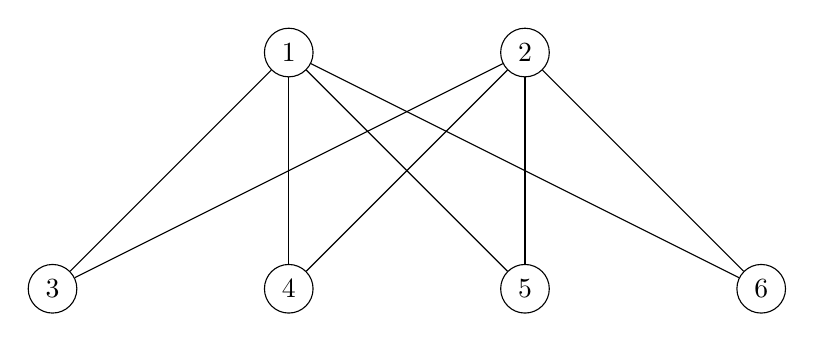
\begin{tikzpicture}[node distance={30mm}, main/.style = {draw, circle}] 
		\node[main] (1) {$1$}; 
		\node[main] (2) [right of=1] {$2$};
		\node[main] (3) [below of=1] {$4$};
		\node[main] (4) [left of=3] {$3$};
		\node[main] (5) [right of=3] {$5$};
		\node[main] (6) [right of=5] {$6$};
		\draw (1) -- (3);
		\draw (1) -- (4);
		\draw (1) -- (5);
		\draw (1) -- (6);
		\draw (2) -- (3);
		\draw (2) -- (4);
		\draw (2) -- (5);
		\draw (2) -- (6);
	\end{tikzpicture}
	\caption{Primjer jednostavnog grafa.}
\end{figure}

Vratimo li se na sliku 1.1, primjetit ćemo da je moguće da vrhove nekog grafa povezuje više bridova, te također da jedan vrh ima brid kojemu je on i početni i krajnji vrh. Takav brid zove se \textit{petlja}. Definicija jednostavnog grafa eliminira mogućnost višestrukih bridova i petlji. Oni će biti od većeg interesa u nastavku ovog rada.

\begin{definition}
	Neka je dan graf G. \textbf{Šetnja} u G je konačan slijed bridova oblika $v_0v_1, v_1v_2, \ldots, v_{m-1}v_m$, također često u oznaci $v_0 \rightarrow v_1 \rightarrow \ldots \rightarrow v_m$, u kojem su svaka dva uzastopna brida ili susjedna ili jednaka.
\end{definition}

Niz različitih bridova $e_1e_2...e_k$ nazivamo \textit{stazom} ako možemo konstruirati šetnju u našem grafu tako da prvo prođemo kroz brid $e_1$, zatim kroz $e_2$ i tako dalje. Važno je da je krajnji vrh brida $e_i$ ujedno i početni vrh brida $e_{i+1}$. Također, ako staza niti jedan vrh ne dotakne dvaput, onda govorimo o \textit{putu}. Ako stazu završimo u istom vrhu u kojem smo započeli te ako smo u konstruiranju staze iskoristili sve bridove od $G$, onda tu stazu nazivamo \textit{eulerovom stazom}. Za takav graf, u kojem postoji šetnja koja počinje i završava u istom grafu, kažemo da sadrži \textit{ciklus}.

Na grafu sa slike 2.1 možemo konstruirati \textit{eulerovu stazu}. 

\begin{figure}[htb]
	\centering
	\begin{tikzpicture}[node distance={30mm}, main/.style = {draw, circle}] 
		\node[main] (1) {$1$}; 
		\node[main] (2) [right of=1] {$2$};
		\node[main] (3) [below of=1] {$3$};
		\node[main] (4) [right of=3] {$4$};
		\node[main] (5) [above left of=1] {$5$};
		\node[main] (6) [below left of=3] {$6$};
		\node[main] (7) [above right of=2] {$7$};
		\node[main] (8) [below right of=4] {$8$};
		\draw (1) -- (3);
		\draw (1) -- (5);
		\draw (1) -- (6);
		\draw (3) -- (5);
		\draw (3) -- (6);
		\draw (2) -- (7);
		\draw (2) -- (4);
		\draw (4) -- (8);
		\draw (7) -- (8);
	\end{tikzpicture}
	\caption{Primjer nepovezanog grafa.}
\end{figure}

\newpage

Na slici 2.2 vidimo graf koji se može promatrati kao unija dva disjunktna grafa. Vidimo da postoje dva vrha između kojih ne možemo konstruirati put (primjerice vrhovi 1 i 2). Ovakve grafove zovemo \textit{nepovezanim grafovima}. U nastavku orijentirat ćemo se na \textit{povezane grafove}.

\begin{definition}
	Ako između svaka dva vrha grafa G postoji put, onda kažemo da je G \textbf{povezan graf}.
\end{definition}

Graf sa slike 2.1 je primjer povezanog grafa.

\begin{definition}
	\textbf{Stupanj vrha} \textit{v} grafa \textit{G} je broj vrhova koji su incidentni s \textit{v}. Označavamo ga s \textit{deg(v)}.
\end{definition}

Za graf sa slike 2.1 vrijedi $deg(1) = deg(2) = 4$ i $deg(3) = deg(4) = deg(5) = deg(6) = 2$.

Također, u nastavku će nam biti važan pojam podgrafa grafa.

\begin{definition}
	\textbf{Podgraf} grafa \textit{G} je graf čiji vrhovi pripadaju skupu $V(G)$ , a bridovi skupu $E(G)$.
\end{definition}

Za graf sa slike 2.1, jedan od podgrafova je i graf na slici 2.3.

\begin{figure}[htb]
	\centering
	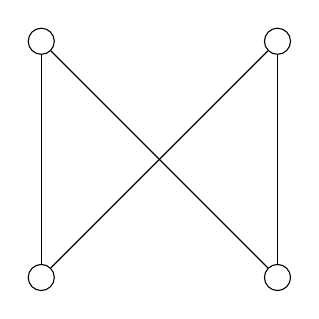
\begin{tikzpicture}[node distance={30mm}, main/.style = {draw, circle}] 
		\node[main] (1) {}; 
		\node[main] (2) [right of=1] {};
		\node[main] (3) [below of=1] {};
		\node[main] (4) [below of=2] {};
		\draw (1) -- (3);
		\draw (1) -- (4);
		\draw (2) -- (3);
		\draw (2) -- (4);
	\end{tikzpicture}
	\caption{Primjer podgrafa grafa sa slike 2.1.}
\end{figure}

\begin{definition}
	Neka je G graf. Izbrišemo li jedan njegov brid, recimo $e$, dobivamo graf $G-e$. Odradimo li postupak konkatenacije nad bridom $e$, dobivamo graf $G \backslash e$.
\end{definition}

\newpage

Nakon što su izneseni neki važni rezultati o samim grafovima, treba se osvrnuti i na njihov prikaz.

\begin{definition}
	Označimo li vrhove zadanog grafa G s ${1, 2, 3,..., n}$, onda definiramo \textbf{matricu susjedstva} $A = [a_{ij}]$ kao $n \times n$ matricu čiji je element $a_{ij}$ jednak broju bridova koji spaja vrh i s vrhom j.
\end{definition}

Za graf sa slike 2.1, pripadna matrica susjedstva je sljedeća:

\[
\centering
A = 
\begin{bmatrix}
	0 & 0 & 1 & 1 & 1 & 1 \\
	0 & 0 & 1 & 1 & 1 & 1\\
	1 & 1 & 0 & 0 & 0 & 0 \\
	1 & 1 & 0 & 0 & 0 & 0 \\
	1 & 1 & 0 & 0 & 0 & 0 \\
	1 & 1 & 0 & 0 & 0 & 0
\end{bmatrix}
\]

Zanimljivo je primjetiti da zbroj svih elemenata u pojedinom retku ili stupcu, točno korespondira stupnju pripadajućeg vrha.

\begin{definition}
	Označe li se dodatno i bridovi zadanog grafa G s ${1, 2, 3, ..., m}$, onda definiramo \textbf{matricu incidencije} kao $n \times m$ matricu $B = [b_{ij}]$ čiji su elementi jednaki 1 ako je vrh 1 incidentan s vrhom j, a 0 inače.
\end{definition}

Za graf sa slike 2.1, pripadajuća matrica incidencije je sljedeća:

\[
\centering
B = 
\begin{bmatrix}
	1 & 1 & 1 & 1 & 0 & 0 & 0 & 0 \\
	0 & 0 & 0 & 0 & 1 & 1 & 1 & 1 \\
	1 & 0 & 0 & 0 & 1 & 0 & 0 & 0 \\
	0 & 1 & 0 & 0 & 0 & 1 & 0 & 0 \\
	0 & 0 & 1 & 0 & 0 & 0 & 1 & 0 \\
	0 & 0 & 0 & 1 & 0 & 0 & 0 & 1
\end{bmatrix}
\]

Sada, kada smo se upoznali s osnovnim pojmovima teorije grafova, uvedimo pojam \textbf{stabla}.

\begin{definition}
	\textbf{Šuma} je graf bez ciklusa, a povezanu šumu zovemo \textbf{stablo}.
\end{definition}

Na slici 2.4 prikazana su tri stabla.

\begin{figure}[htb]
	\minipage{0.33\textwidth}
	\begin{center}
		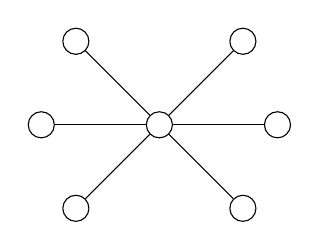
\begin{tikzpicture}[node distance={15mm}, main/.style = {draw, circle}] 
			\node[main] (1) {}; 
			\node[main] (2) [above left of=1] {};
			\node[main] (3) [above right of=1] {};
			\node[main] (4) [right of=1] {};
			\node[main] (5) [below right of=1] {};
			\node[main] (6) [below left of=1] {};
			\node[main] (7) [left of=1] {};
			\draw (1) -- (2);
			\draw (1) -- (3);
			\draw (1) -- (4);
			\draw (1) -- (5);
			\draw (1) -- (6);
			\draw (1) -- (7);
		\end{tikzpicture}
	\end{center}
	\endminipage\hfill
	\minipage{0.33\textwidth}
	\begin{center}
		\begin{tikzpicture}[node distance={15mm}, main/.style = {draw, circle}] 
			\node[main] (1) {}; 
			\node[main] (2) [below of=1] {};
			\node[main] (3) [right of=1] {};
			\node[main] (4) [right of=2] {};
			\node[main] (5) [above of=3] {};
			\node[main] (6) [below of=4] {};
			\node[main] (7) [below right of=5] {};
			\node[main] (8) [above right of=6] {};
			\node[main] (9) [below right of=7] {};
			\draw (1) -- (3);
			\draw (2) -- (4);
			\draw (5) -- (7);
			\draw (6) -- (8);
			\draw (8) -- (9);
			\draw (7) -- (9);
			\draw (3) -- (7);
			\draw (4) -- (8);
		\end{tikzpicture}
	\end{center}
	\endminipage\hfill
	\minipage{0.33\textwidth}
	\begin{center}
		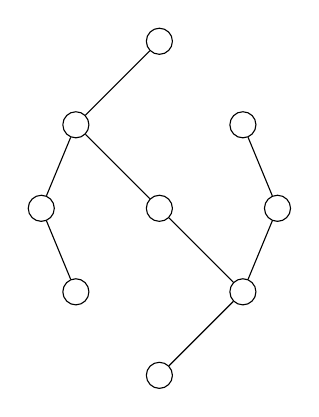
\begin{tikzpicture}[node distance={15mm}, main/.style = {draw, circle}] 
			\node[main] (1) {}; 
			\node[main] (2) [above left of=1] {};
			\node[main] (3) [above right of=1] {};
			\node[main] (4) [right of=1] {};
			\node[main] (5) [below right of=1] {};
			\node[main] (6) [below left of=1] {};
			\node[main] (7) [left of=1] {};
			\node[main] (8) [below right of=6] {};
			\node[main] (9) [above right of=2] {};
			\draw (1) -- (2);
			\draw (1) -- (5);
			\draw (3) -- (4);
			\draw (4) -- (5);
			\draw (2) -- (7);
			\draw (6) -- (7);
			\draw (5) -- (8);
			\draw (2) -- (9);
		\end{tikzpicture}
	\end{center}
	\endminipage\hfill
	\caption{Primjeri stabala.}
\end{figure}

Primjetimo da svako stablo s $n$ vrhova ima točno $n - 1$ bridova.

\begin{theorem}[Broj bridova stabala]
	Sva stabla s $n$ vrhova imaju $n-1$ bridova. Posljedično, svi povezani grafovi s $n$ vrhova i $n-1$ bridova su stabla.
\end{theorem}

Prije dokaza ovog teorema potrebno je uvesti jednu lemmu.

\begin{lemma}
	Neka je $T$ stablo s $n$ vrhova, gdje je $n >= 2$. Tada $T$ ima barem $2$ vrha čiji je stupanj jednak $1$.
\end{lemma}

\begin{proof}
	Uzmimo proizvoljni put \textit{p} maksmimalne dužine u grafu $T$. Tada kranje točke puta $p$ moraju biti listovi. Pretpostavimo li da jedan od ta dva vrha, recimo $a$, nije list, tada $p$ može biti produžen s barem jednim bridom koji nije dio puta $p$, a incidentan je s $a$, što znači da taj put nije maksimalne duljine.
\end{proof}

Vrhove stabla čiji je stupanj jednak 1 zovemo \textit{listovi}. Sada možemo dokazati teorem 2.8.

\begin{proof}
	Koristimo matematičku indukciju na broju vrhova $n$. Ako je $n = 1$, tvrdnja je trivijalno istinita jer neciklički graf s $1$ vrhom nema bridova. Pretpostavimo da je tvrdnja istinita za stabla s $n$ vrhova. Neka je $T$ stablo s $n + 1$ vrhova. Pretpostavimo da je vrh $l$ list stabla $T$ (lemma 2.9 nam govori da list postoji), te obrišimo vrh $l$ i brid $e$ koji je s njim incidentan. Dobit ćemo novo stablo $T'$. (Primjetimo da će $T'$ uvijek biti stablo budući da je povezan, i ne sadrži ciklus.) $T'$ ima $n$ vrhova, te po pretpostavci ima $n-1$ bridova. Sada $T = T' \cup e$ ima n vrhova, i teorem je dokazan.
\end{proof} 

Sada smo se upoznali sa pojmom stabla. U nastavku će biti više govora o \textbf{razapinjućim stablima}. Također, u nastavku će nas zanimati samo jednostavni i povezani grafovi, tako da to neću svaki put eksplicitno naglašavati.

\chapter{Razapinjuća stabla}

\begin{definition}
	\textbf{Razapinjući podgraf} zadanog grafa $G = (V, E)$ s $n$ vrhova je svaki podgraf $G' = (V, E')$ grafa $G$ s istim skupom vrhova kao i $G$.
\end{definition}

\begin{figure}[htb]
	\minipage{0.5\textwidth}
	\begin{center}
		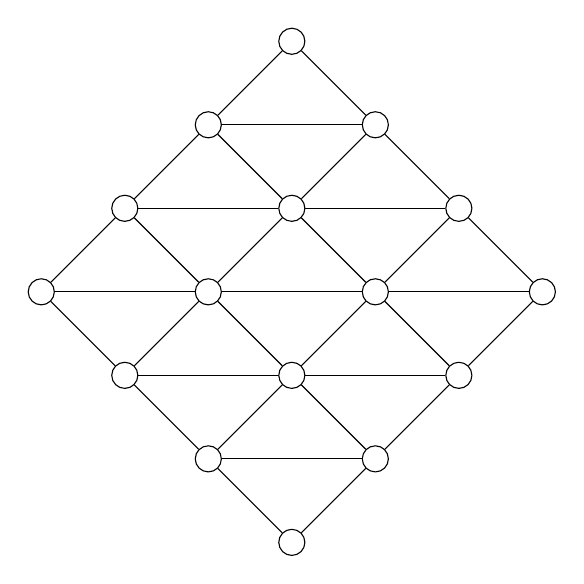
\begin{tikzpicture}[node distance={15mm}, main/.style = {draw, circle}] 
			\node[main] (1) {}; 
			\node[main] (2) [above left of=1] {};
			\node[main] (3) [below left of=1] {};
			\node[main] (4) [above right of=2] {};
			\node[main] (5) [below right of=3] {};
			\node[main] (6) [above right of=4] {};
			\node[main] (7) [above right of=1] {};
			\node[main] (8) [below right of=1] {};
			\node[main] (9) [below right of=5] {};
			\node[main] (10) [above right of=9] {};
			\node[main] (11) [below right of=6] {};
			\node[main] (12) [above right of=8] {};
			\node[main] (13) [above right of=12] {};
			\node[main] (14) [below right of=12] {};
			\node[main] (15) [below left of=2] {};
			\node[main] (16) [above right of=14] {};
			\draw (1) -- (8);
			\draw (1) -- (7);
			\draw (7) -- (12);
			\draw (1) -- (15);
			\draw (1) -- (2);
			\draw (1) -- (3);
			\draw (4) -- (7);
			\draw (12) -- (13);
			\draw (11) -- (13);
			\draw (4) -- (6);
			\draw (13) -- (16);
			\draw (5) -- (9);
			\draw (9) -- (10);
			\draw (8) -- (10);
			\draw (10) -- (14);
			\draw (8) -- (12);
			\draw (1) -- (12);
			\draw (7) -- (13);
			\draw (7) -- (11);
			\draw (4) -- (11);
			\draw (6) -- (11);
			\draw (2) -- (4);
			\draw (2) -- (7);
			\draw (2) -- (15);
			\draw (3) -- (15);
			\draw (3) -- (5);
			\draw (3) -- (8);
			\draw (5) -- (8);
			\draw (5) -- (10);
			\draw (8) -- (14);
			\draw (12) -- (14);
			\draw (12) -- (16);
			\draw (14) -- (16);
		\end{tikzpicture}
	\end{center}
	\endminipage\hfill
	\minipage{0.5\textwidth}
	\begin{center}
		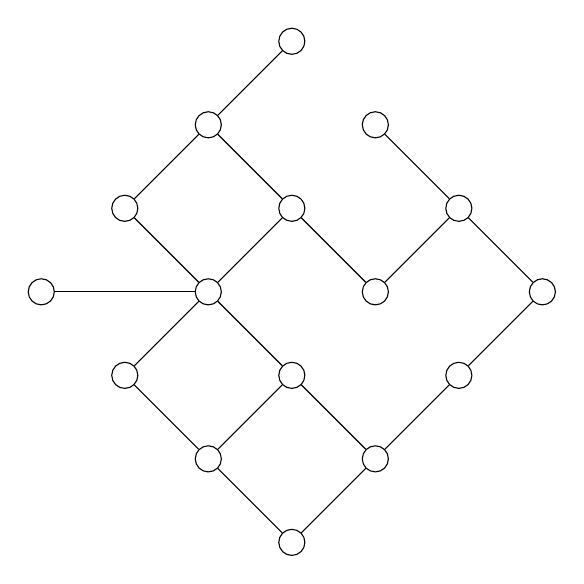
\begin{tikzpicture}[node distance={15mm}, main/.style = {draw, circle}] 
			\node[main] (1) {}; 
			\node[main] (2) [above left of=1] {};
			\node[main] (3) [below left of=1] {};
			\node[main] (4) [above right of=2] {};
			\node[main] (5) [below right of=3] {};
			\node[main] (6) [above right of=4] {};
			\node[main] (7) [above right of=1] {};
			\node[main] (8) [below right of=1] {};
			\node[main] (9) [below right of=5] {};
			\node[main] (10) [above right of=9] {};
			\node[main] (11) [below right of=6] {};
			\node[main] (12) [above right of=8] {};
			\node[main] (13) [above right of=12] {};
			\node[main] (14) [below right of=12] {};
			\node[main] (15) [below left of=2] {};
			\node[main] (16) [above right of=14] {};
			\draw (1) -- (8);
			\draw (1) -- (7);
			\draw (7) -- (12);
			\draw (1) -- (15);
			\draw (1) -- (2);
			\draw (1) -- (3);
			\draw (4) -- (7);
			\draw (12) -- (13);
			\draw (11) -- (13);
			\draw (4) -- (6);
			\draw (13) -- (16);
			\draw (5) -- (9);
			\draw (10) -- (9);
			\draw (10) -- (8);
			\draw (10) -- (14);
			\draw (2) -- (4);
			\draw (3) -- (5);
			\draw (5) -- (8);
			\draw (14) -- (16);
		\end{tikzpicture}
	\end{center}
	\endminipage\hfill
	\caption{Primjer grafa i jednog njegovog razapinjućeg podgrafa.}
\end{figure}

Na primjeru sa slike 3.1 lako je uočiti da razapinjući podgraf zadanog grafa nije jedinstven.

\begin{definition}
	\textbf{Razapinjuće stablo} zadanog grafa $G = (V, E)$ s $n$ vrhova je podgraf $G' = (V, E')$ grafa $G$ koji je ujedno i stablo.
\end{definition}

Primjer razapinjućeg stabla za graf sa slike 3.1 je na slici 3.2.

\newpage

\begin{figure}[htb]
	\centering
	\begin{tikzpicture}[node distance={15mm}, main/.style = {draw, circle}] 
		\node[main] (1) {}; 
		\node[main] (2) [above left of=1] {};
		\node[main] (3) [below left of=1] {};
		\node[main] (4) [above right of=2] {};
		\node[main] (5) [below right of=3] {};
		\node[main] (6) [above right of=4] {};
		\node[main] (7) [above right of=1] {};
		\node[main] (8) [below right of=1] {};
		\node[main] (9) [below right of=5] {};
		\node[main] (10) [above right of=9] {};
		\node[main] (11) [below right of=6] {};
		\node[main] (12) [above right of=8] {};
		\node[main] (13) [above right of=12] {};
		\node[main] (14) [below right of=12] {};
		\node[main] (15) [below left of=2] {};
		\node[main] (16) [above right of=14] {};
		\draw (1) -- (8);
		\draw (1) -- (7);
		\draw (7) -- (12);
		\draw (1) -- (15);
		\draw (1) -- (2);
		\draw (1) -- (3);
		\draw (4) -- (7);
		\draw (12) -- (13);
		\draw (11) -- (13);
		\draw (4) -- (6);
		\draw (13) -- (16);
		\draw (5) -- (9);
		\draw (10) -- (9);
		\draw (10) -- (8);
		\draw (10) -- (14);
	\end{tikzpicture}
	\caption{Jedno razapinjuće stablo grafa sa slike 3.1.}
\end{figure}

Naravno, stablo sa slike 3.2 nije jedino razapinjuće stablo grafa sa slike 3.1. Bridovima zadanog grafa možemo pridružiti težine. Tada govorimo o težinskom grafu. Problem određivanja minimalnog razapinjućeg stabla težinskog grafa ima brojne primjene.

\section{Minimalna razapinjuća stabla grafa}

Pretpostavimo da djelatnici Hrvatskih Autocesta žele sagraditi autoceste koje će povezivati gradove Zagreb $(Z)$, Sisak $(S)$, Kutinu, $(K)$, Glinu $(G)$ te Novsku $(N)$. Graf koji prikazuje odnose između ovih gradova prikazan je na slici 3.3. Cilj je povezati sve gradove s autocestom, no s obzirom da je izgradnja skupa, žele se povezati svi gradovi tako da ukupna kilometraža novih cesta bude najmanja moguća. Rješenje ovog problema je u pronalasku minimalnog razapinjućeg stabla. Poznato je nekoliko algoritama, istaknimo \textbf{Primov algoritam}, koji se svodi na to da odaberemo proizvoljni vrh grafa, pa se od skupa ostalih vrhova bira onaj koji je s odabranim vrhom susjedan, te čiji incidentni brid ima najmanju težinu. Svakim korakom algoritma tako povećavamo skup odabranih vrhova, i algoritam se ponavlja dok kardinalni broj odabranih vrhova ne bude jednak broju vrhova grafa. Rezultat će biti najmanje razapinjuće stablo zadanog grafa.

\begin{algorithm}
	\caption{Primov algoritam}
	\label{algo:prim-algorithm}
	\begin{algorithmic}
		\STATE{\textbf{Ulaz:} težinski, neusmjereni graf $G = (V, E, w)$.}
		\STATE{\textbf{Izlaz:} minimalno razapinjuće stablo $T$.}
		\STATE{$T \leftarrow \emptyset $}
		\STATE{Neka je $r$ proizvoljno odabran vrh iz $V$.}
		\STATE{$U \leftarrow \{r\} $}	
		\WHILE{($\arrowvert U \arrowvert < n$)}
			\STATE{Pronađi $u \in U$ i $v \in V - U$ takve da je brid $(u, v)$ minimalni brid između $U$ i $V - U$.}
			\STATE{$T\leftarrow T \cup \{(u, v)\}$}
			\STATE{$U \cup \{v\}$}
		\ENDWHILE
		\RETURN{$T$}
	\end{algorithmic}
\end{algorithm}

\newpage

\begin{figure}[htb]
	\centering
	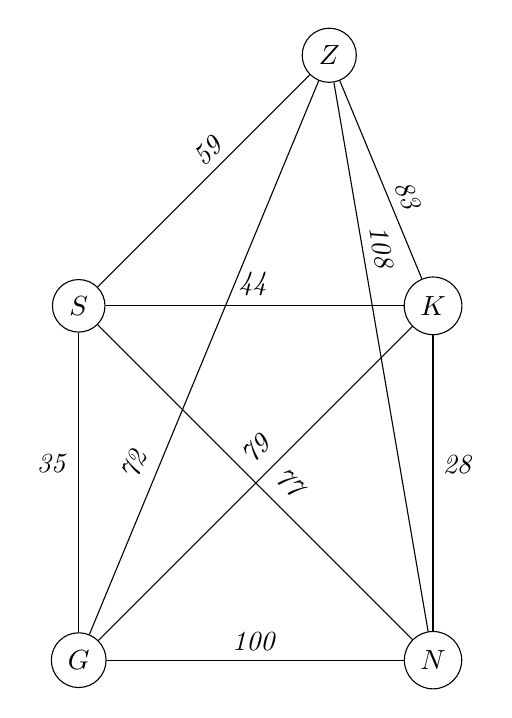
\begin{tikzpicture}[node distance={45mm}, main/.style = {draw, circle}] 
		\node[main] (1) {$S$}; 
		\node[main] (2) [right of=1] {$K$};
		\node[main] (3) [below of=1] {$G$};
		\node[main] (4) [below of=2] {$N$};
		\node[main] (5) [above right of=1] {$Z$};
		\draw (1) -- node[midway, above right, sloped] {\textit{77}} (4);
		\draw (2) -- node[midway, above right, sloped] {\textit{79}} (3);
		\draw (1) -- node[midway, above] {\textit{44}} (2);
		\draw (1) -- node[midway, above left] {\textit{35}} (3);
		\draw (2) -- node[midway, above right] {\textit{28}} (4);
		\draw (3) -- node[midway, above] {\textit{100}} (4);
		\draw (1) -- node[midway, above right, sloped] {\textit{59}} (5);
		\draw (2) -- node[midway, above right, sloped] {\textit{83}} (5);
		\draw (3) -- node[midway, above right, sloped, pos=0.25] {\textit{72}} (5);
		\draw (5) -- node[midway, above right, sloped, pos=0.25] {\textit{108}} (4);
	\end{tikzpicture}
	\caption{Graf koji prikazuje odnose između gradova. Težina brida predstavlja udaljenost između dva pripadajuća grada izraženu u kilometrima.}
\end{figure}

Minimalno razapinjuće stablo grafa sa slike 3.3, prikazano je na slici 3.4.

\begin{figure}[htb]
	\centering
	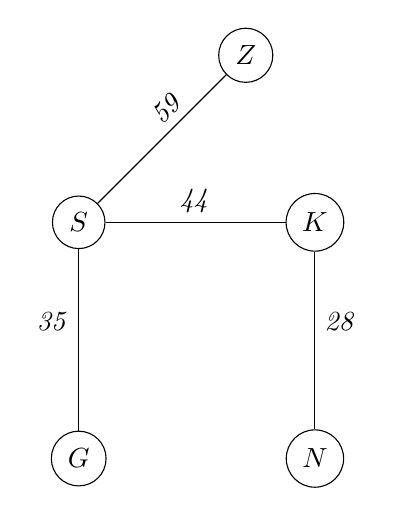
\begin{tikzpicture}[node distance={30mm}, main/.style = {draw, circle}] 
		\node[main] (1) {$S$}; 
		\node[main] (2) [right of=1] {$K$};
		\node[main] (3) [below of=1] {$G$};
		\node[main] (4) [below of=2] {$N$};
		\node[main] (5) [above right of=1] {$Z$};
		\draw (1) -- node[midway, above] {\textit{44}} (2);
		\draw (1) -- node[midway, above left] {\textit{35}} (3);
		\draw (2) -- node[midway, above right] {\textit{28}} (4);
		\draw (1) -- node[midway, above right, sloped] {\textit{59}} (5);
	\end{tikzpicture}
	\caption{Minimalno razapinjuće stablo grafa sa slike 3.3}
\end{figure}

\newpage

Ovaj problem iz teorije grafova može se dovesti u vezu i s drugim problemima iz industrije. Primjenom opisanog rješenja može se uštedjeti pri konstrukciji železničke mreže. Također, ako se u neki grad želi uvesti kabelska televizija, djelatnici će  upravo traženjem minimalnog razapinjućeg stabla tražiti najbolji način za povezati svaki dio grafa sa kablovima. Pri dizajnu električnih krugova, potrebno je povezati određene točke da bi bile električki ekvivalentne. Korištenje minimalnog razapinjućeg stabla omogućit će minimalno korištenje žice. Ovo su samo neke od mogućih primjena.

U nastavku rada nećemo konstruirati razapinjuća stabla zadanog grafa, već ćemo se baviti pitanjem koliko razapinjućih stabala neki graf $G$ uopće ima. Odgovor na postavljeno pitanje nije jednostavan i ne postoji zatvorena formula za broj razapinjućih stabala zadanog grafa.

\newpage

\section{Primjeri prebrojavanja razapinjućih stabala grafa}

U ovom odjeljku bavit ću se određivanjem eksplicitnih formula za računanje broja razapinjućih stabala određenih familija grafova.

Za grafove s malim brojem vrhova mogu se i na prste konstruirati sva razapinjuća stabla, no već i za grafove s 5 vrhova i nemalim brojem bridova (jednostavni graf s $n$ vrhova može imati maksimalno $\binom{n}{2}$ bridova) taj problem postaje prekompleksan i zahtjeva sistematičniji pristup.

\begin{figure}[htb]
	\centering
	\begin{tikzpicture}[node distance={30mm}, main/.style = {draw, circle}] 
		\node[main] (1) {}; 
		\node[main] (2) [above right of=1] {};
		\node[main] (3) [above left of=1] {};
		\node[main] (4) [below left of=1] {};
		\node[main] (5) [below right of=1] {};
		\draw (1) -- (2);
		\draw (1) -- (4);
		\draw (2) -- (3);
		\draw (2) -- (5);
		\draw (3) -- (4);
		\draw (4) -- (5);
	\end{tikzpicture}
	\caption{Primjer grafa}
\end{figure}

Na slici 3.5 prikazan je jednostavan graf s 5 vrhova, a na slici 3.6 prikazano je njegovih 12 razapinjućih stabala.

\begin{figure}[htb]
	\minipage{0.25\textwidth}
	\begin{center}
		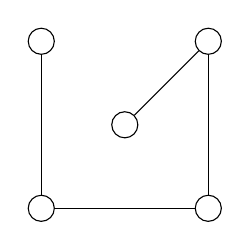
\begin{tikzpicture}[node distance={15mm}, main/.style = {draw, circle}] 
			\node[main] (1) {}; 
			\node[main] (2) [above right of=1] {};
			\node[main] (3) [above left of=1] {};
			\node[main] (4) [below left of=1] {};
			\node[main] (5) [below right of=1] {};
			\draw (1) -- (2);
			\draw (2) -- (5);
			\draw (3) -- (4);
			\draw (4) -- (5);
		\end{tikzpicture}
	\end{center}
	\endminipage\hfill
	\minipage{0.25\textwidth}
	\begin{center}
		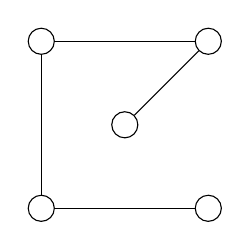
\begin{tikzpicture}[node distance={15mm}, main/.style = {draw, circle}] 
			\node[main] (1) {}; 
			\node[main] (2) [above right of=1] {};
			\node[main] (3) [above left of=1] {};
			\node[main] (4) [below left of=1] {};
			\node[main] (5) [below right of=1] {};
			\draw (1) -- (2);
			\draw (2) -- (3);
			\draw (3) -- (4);
			\draw (4) -- (5);
		\end{tikzpicture}
	\end{center}
	\endminipage\hfill
	\minipage{0.25\textwidth}
	\begin{center}
		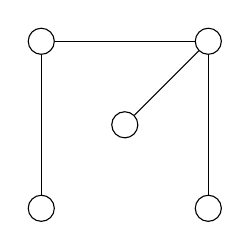
\begin{tikzpicture}[node distance={15mm}, main/.style = {draw, circle}] 
			\node[main] (1) {}; 
			\node[main] (2) [above right of=1] {};
			\node[main] (3) [above left of=1] {};
			\node[main] (4) [below left of=1] {};
			\node[main] (5) [below right of=1] {};
			\draw (1) -- (2);
			\draw (2) -- (3);
			\draw (2) -- (5);
			\draw (3) -- (4);
		\end{tikzpicture}
	\end{center}
	\endminipage\hfill
	\minipage{0.25\textwidth}
	\begin{center}
		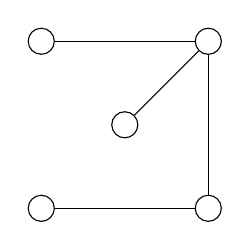
\begin{tikzpicture}[node distance={15mm}, main/.style = {draw, circle}] 
			\node[main] (1) {}; 
			\node[main] (2) [above right of=1] {};
			\node[main] (3) [above left of=1] {};
			\node[main] (4) [below left of=1] {};
			\node[main] (5) [below right of=1] {};
			\draw (1) -- (2);
			\draw (2) -- (3);
			\draw (2) -- (5);
			\draw (4) -- (5);
		\end{tikzpicture}
	\end{center}
	\endminipage\hfill
	\minipage{0.25\textwidth}
	\begin{center}
		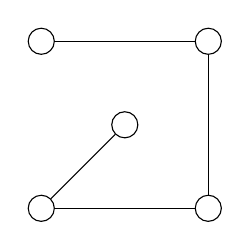
\begin{tikzpicture}[node distance={15mm}, main/.style = {draw, circle}] 
			\node[main] (1) {}; 
			\node[main] (2) [above right of=1] {};
			\node[main] (3) [above left of=1] {};
			\node[main] (4) [below left of=1] {};
			\node[main] (5) [below right of=1] {};
			\draw (1) -- (4);
			\draw (2) -- (3);
			\draw (2) -- (5);
			\draw (4) -- (5);
		\end{tikzpicture}
	\end{center}
	\endminipage\hfill
	\minipage{0.25\textwidth}
	\begin{center}
		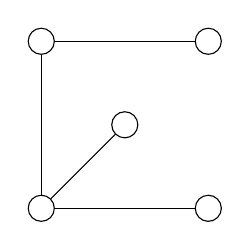
\begin{tikzpicture}[node distance={15mm}, main/.style = {draw, circle}] 
			\node[main] (1) {}; 
			\node[main] (2) [above right of=1] {};
			\node[main] (3) [above left of=1] {};
			\node[main] (4) [below left of=1] {};
			\node[main] (5) [below right of=1] {};
			\draw (1) -- (4);
			\draw (2) -- (3);
			\draw (3) -- (4);
			\draw (4) -- (5);
		\end{tikzpicture}
	\end{center}
	\endminipage\hfill
	\minipage{0.25\textwidth}
	\begin{center}
		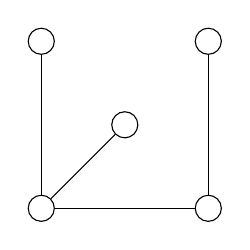
\begin{tikzpicture}[node distance={15mm}, main/.style = {draw, circle}] 
			\node[main] (1) {}; 
			\node[main] (2) [above right of=1] {};
			\node[main] (3) [above left of=1] {};
			\node[main] (4) [below left of=1] {};
			\node[main] (5) [below right of=1] {};
			\draw (1) -- (4);
			\draw (2) -- (5);
			\draw (3) -- (4);
			\draw (4) -- (5);
		\end{tikzpicture}
	\end{center}
	\endminipage\hfill
	\minipage{0.25\textwidth}
	\begin{center}
		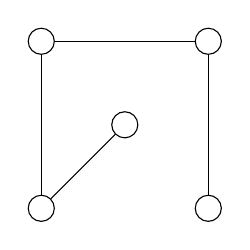
\begin{tikzpicture}[node distance={15mm}, main/.style = {draw, circle}] 
			\node[main] (1) {}; 
			\node[main] (2) [above right of=1] {};
			\node[main] (3) [above left of=1] {};
			\node[main] (4) [below left of=1] {};
			\node[main] (5) [below right of=1] {};
			\draw (1) -- (4);
			\draw (2) -- (3);
			\draw (2) -- (5);
			\draw (3) -- (4);
		\end{tikzpicture}
	\end{center}
	\endminipage\hfill
	\minipage{0.25\textwidth}
	\begin{center}
		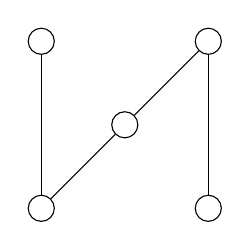
\begin{tikzpicture}[node distance={15mm}, main/.style = {draw, circle}] 
			\node[main] (1) {}; 
			\node[main] (2) [above right of=1] {};
			\node[main] (3) [above left of=1] {};
			\node[main] (4) [below left of=1] {};
			\node[main] (5) [below right of=1] {};
			\draw (1) -- (2);
			\draw (1) -- (4);
			\draw (2) -- (5);
			\draw (3) -- (4);
		\end{tikzpicture}
	\end{center}
	\endminipage\hfill
	\minipage{0.25\textwidth}
	\begin{center}
		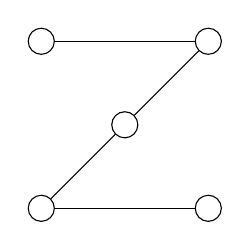
\begin{tikzpicture}[node distance={15mm}, main/.style = {draw, circle}] 
			\node[main] (1) {}; 
			\node[main] (2) [above right of=1] {};
			\node[main] (3) [above left of=1] {};
			\node[main] (4) [below left of=1] {};
			\node[main] (5) [below right of=1] {};
			\draw (1) -- (2);
			\draw (1) -- (4);
			\draw (2) -- (3);
			\draw (4) -- (5);
		\end{tikzpicture}
	\end{center}
	\endminipage\hfill
	\minipage{0.25\textwidth}
	\begin{center}
		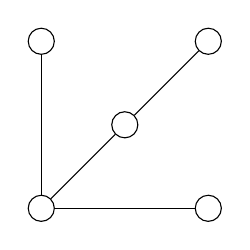
\begin{tikzpicture}[node distance={15mm}, main/.style = {draw, circle}] 
			\node[main] (1) {}; 
			\node[main] (2) [above right of=1] {};
			\node[main] (3) [above left of=1] {};
			\node[main] (4) [below left of=1] {};
			\node[main] (5) [below right of=1] {};
			\draw (1) -- (2);
			\draw (1) -- (4);
			\draw (3) -- (4);
			\draw (4) -- (5);
		\end{tikzpicture}
	\end{center}
	\endminipage\hfill
	\minipage{0.25\textwidth}
	\begin{center}
		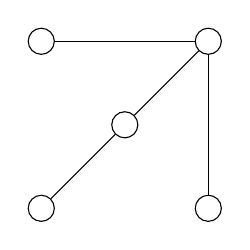
\begin{tikzpicture}[node distance={15mm}, main/.style = {draw, circle}] 
			\node[main] (1) {}; 
			\node[main] (2) [above right of=1] {};
			\node[main] (3) [above left of=1] {};
			\node[main] (4) [below left of=1] {};
			\node[main] (5) [below right of=1] {};
			\draw (1) -- (2);
			\draw (1) -- (4);
			\draw (2) -- (3);
			\draw (2) -- (5);
		\end{tikzpicture}
	\end{center}
	\endminipage\hfill
	\caption{Razapinjuća stabla grafa sa slike 3.5}
\end{figure}

\newpage

Kao što vidimo, već za graf sa slike 3.5, koji ima 5 vrhova i 6 bridova (grafovi s 5 vrhova mogu imati maksimalno 10 bridova) ima 12 razapinjućih stabala. Očigledno je da će se povećanjem broja bridova i broja vrhova ovaj zadatak čovjeku znatno otežati, i tu se rađa potreba za pametnijim načinom računanja.

\subsection{Kotač \textit{W\textsubscript{n}}}

Prvi primjer je graf kotač. Kotač $W_n$ je graf koji se dobije iz ciklusa $C_n$ dodavanjem još jednog vrha povezanog sa svim vrhovima ciklusa.

\begin{figure}[htb]
	\centering
	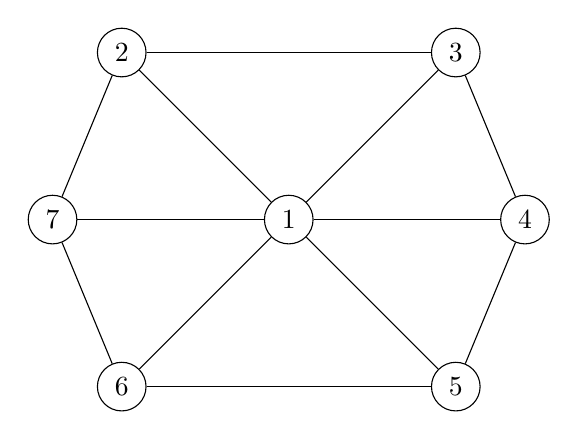
\begin{tikzpicture}[node distance={30mm}, main/.style = {draw, circle}] 
		\node[main] (1) {$1$}; 
		\node[main] (2) [above left of=1] {$2$};
		\node[main] (3) [above right of=1] {$3$};
		\node[main] (4) [right of=1] {$4$};
		\node[main] (5) [below right of=1] {$5$};
		\node[main] (6) [below left of=1] {$6$};
		\node[main] (7) [left of=1] {$7$};
		\draw (1) -- (2);
		\draw (1) -- (3);
		\draw (1) -- (4);
		\draw (1) -- (5);
		\draw (1) -- (6);
		\draw (1) -- (7);
		\draw (2) -- (3);
		\draw (3) -- (4);
		\draw (4) -- (5);
		\draw (5) -- (6);
		\draw (6) -- (7);
		\draw (7) -- (2);
	\end{tikzpicture}
	\caption{Kotač $W_6$.}
\end{figure}

Jedan primjer kotača je i $W_6$ prikazan na slici 3.1. Odredit ćemo ukupan broj razapinjućih stabala kotača $W_n$.

\begin{proposition}
	 Neka je $T(G)$ broj razapinjućih stabala grafa $G$. Vrijedi:
	\begin{equation}
		T(G) = T(G - e) + T(G \backslash e)
	\end{equation}
\end{proposition}

Prije samog izračuna, potrebno je dokazati propoziciju 3.5.

\begin{proof}
Neka je \textit{e} neki fiksni brid od \textit{G}. Uočimo da se razapinjuća stabla od \textit{G} dijele na:
\begin{itemize}
	\item razapinjuća stabla od \textit{G} koja ne sadrže brid \textit{e}; neka je taj broj jednak x,
	\item razapinjuća stabla od \textit{G} koja sadrže brid \textit{e}; neka je taj broj jednak y.
\end{itemize}
Vrijedi: $T(G) = x + y$. Uočimo sada da je:
\begin{itemize}
	\item $x = T(G - e)$ jer je svako razapinjuće stablo od \textit{G} koje ne sadrži \textit{e}, ujedno i razapinjuće stablo od $G - e$
	\item $y = T(G \backslash e)$ jer svako razapinjuće stablo od $G \backslash e$ možemo dobiti iz razapinjućeg stabla od \textit{G} koje sadrži brid \textit{e} postupkom konkatenacije brida \textit{e} u tom stablu.
\end{itemize}
Dakle, vrijedi $T(G) = T(G - e) + T(G \backslash e)$.\footnote{Dokaz po uzoru na \cite{MM}}
\end{proof}

Da bismo mogli pronaći eksplicitnu formulu za računanje broja razapinjućih stabala kotača s proizvoljnim brojem vrhova, potrebno je definirati nekoliko familija grafova koje ćemo koristiti: $A_n$, $B_n$, $C_n$\footnote{$C_n$ u ovom primjeru, iznimno, neće označavati ciklus} i $D_n$.

\begin{figure}[htb]
	\minipage{0.33\textwidth}
	\begin{center}
		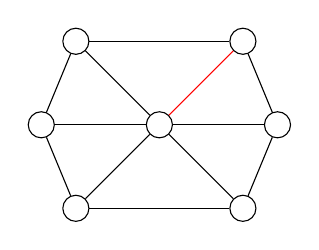
\begin{tikzpicture}[node distance={15mm}, main/.style = {draw, circle}] 
			\node[main] (1) {}; 
			\node[main] (2) [above left of=1] {};
			\node[main] (3) [above right of=1] {};
			\node[main] (4) [right of=1] {};
			\node[main] (5) [below right of=1] {};
			\node[main] (6) [below left of=1] {};
			\node[main] (7) [left of=1] {};
			\draw (1) -- (2);
			\draw[red] (1) -- (3);
			\draw (1) -- (4);
			\draw (1) -- (5);
			\draw (1) -- (6);
			\draw (1) -- (7);
			\draw (2) -- (3);
			\draw (3) -- (4);
			\draw (4) -- (5);
			\draw (5) -- (6);
			\draw (6) -- (7);
			\draw (7) -- (2);
		\end{tikzpicture}
	\end{center}
	\caption*{\textit{$W_n$}}
	\endminipage\hfill
	\minipage{0.33\textwidth}
	\begin{center}
		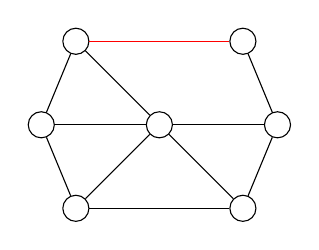
\begin{tikzpicture}[node distance={15mm}, main/.style = {draw, 	circle}] 
			\node[main] (1) {}; 
			\node[main] (2) [above left of=1] {};
			\node[main] (3) [above right of=1] {};
			\node[main] (4) [right of=1] {};
			\node[main] (5) [below right of=1] {};
			\node[main] (6) [below left of=1] {};
			\node[main] (7) [left of=1] {};
			\draw (1) -- (2);
			\draw (1) -- (4);
			\draw (1) -- (5);
			\draw (1) -- (6);
			\draw (1) -- (7);
			\draw[red] (2) -- (3);
			\draw (3) -- (4);
			\draw (4) -- (5);
			\draw (5) -- (6);
			\draw (6) -- (7);
			\draw (7) -- (2);
		\end{tikzpicture}
	\end{center}
	\caption*{$A_n$}
	\endminipage\hfill
	\minipage{0.33\textwidth}
	\begin{center}
		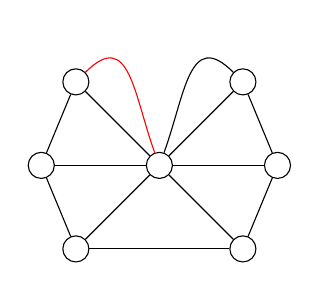
\begin{tikzpicture}[node distance={15mm}, main/.style = {draw, 	circle}] 
			\node[main] (1) {}; 
			\node[main] (2) [above left of=1] {};
			\node[main] (3) [above right of=1] {};
			\node[main] (4) [right of=1] {};
			\node[main] (5) [below right of=1] {};
			\node[main] (6) [below left of=1] {};
			\node[main] (7) [left of=1] {};
			\draw (1) -- (2);
			\draw (1) -- (3);
			\draw (1) -- (4);
			\draw[red] (1) to [out=110,in=45,looseness=1.5] (2);
			\draw (1) to [out=70,in=135,looseness=1.5] (3);
			\draw (1) -- (5);
			\draw (1) -- (6);
			\draw (1) -- (7);
			\draw (3) -- (4);
			\draw (4) -- (5);
			\draw (5) -- (6);
			\draw (6) -- (7);
			\draw (7) -- (2);
		\end{tikzpicture}
	\end{center}
	\caption*{$B_n$}
	\endminipage\hfill
	\minipage{0.5\textwidth}
	\begin{center}
		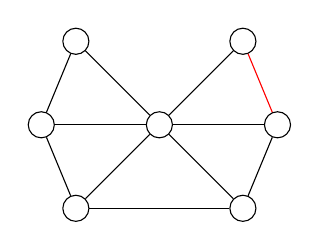
\begin{tikzpicture}[node distance={15mm}, main/.style = {draw, 	circle}] 
			\node[main] (1) {}; 
			\node[main] (2) [above left of=1] {};
			\node[main] (3) [above right of=1] {};
			\node[main] (4) [right of=1] {};
			\node[main] (5) [below right of=1] {};
			\node[main] (6) [below left of=1] {};
			\node[main] (7) [left of=1] {};
			\draw (1) -- (2);
			\draw (1) -- (3);
			\draw (1) -- (4);
			\draw (1) -- (5);
			\draw (1) -- (6);
			\draw (1) -- (7);
			\draw[red] (3) -- (4);
			\draw (4) -- (5);
			\draw (5) -- (6);
			\draw (6) -- (7);
			\draw (7) -- (2);
		\end{tikzpicture}
	\end{center}
	\caption*{$C_n$}
	\endminipage\hfill
	\minipage{0.5\textwidth}
	\begin{center}
		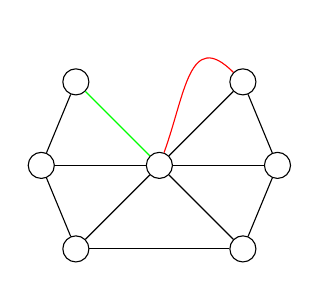
\begin{tikzpicture}[node distance={15mm}, main/.style = {draw, 	circle}] 
			\node[main] (1) {}; 
			\node[main] (2) [above left of=1] {};
			\node[main] (3) [above right of=1] {};
			\node[main] (4) [right of=1] {};
			\node[main] (5) [below right of=1] {};
			\node[main] (6) [below left of=1] {};
			\node[main] (7) [left of=1] {};
			\draw[green] (1) -- (2);
			\draw (1) -- (3);
			\draw (1) -- (4);
			\draw[red] (1) to [out=70,in=135,looseness=1.5] (3);
			\draw (1) -- (5);
			\draw (1) -- (6);
			\draw (1) -- (7);
			\draw (3) -- (4);
			\draw (4) -- (5);
			\draw (5) -- (6);
			\draw (6) -- (7);
			\draw (7) -- (2);
		\end{tikzpicture}
	\end{center}
	\caption*{$D_n$}
	\endminipage\hfill
	\caption{Pet familija grafova koje će se koristiti za nalaženje eksplicitne formule za računanje broja razapinjućih stabala grafa kotača $W_n$ ($n$ označava broj vrhova).}
\end{figure}

Graf $A_n$ dobivamo iz $W_n$ brisanjem jednog od bridova s kojima je "centralni" vrh kotača povezan s vrhovima ciklusa. (Na slici 3.8 taj je brid od $W_n$ označen crvenom bojom.) $B_n$ se dobije ako taj isti brid iz $W_n$ obrišemo postupkom kontrakcije. $C_n$ dobivamo iz $W_n$ tako da obrišemo jedan brid između vrhova ciklusa. $D_n$ dobivamo iz $B_n$. Primjetimo da u $B_n$ postoje dva vrha koja sa "centralnim" vrhom imaju višestruke bridove. $D_n$ ćemo dobiti ako obrišemo jedan od tih bridova.

\newpage

Koristimo izraz (3.1) nad označenim bridovima sa slike 3.2, te dobivamo sustav rekurzivnih relacija:

$T(W_n) = T(A_n) + T(B_{n - 1})$

$T(A_n) = T(C_{n - 1}) + T(W_{n - 1})$

$T(B_n) = T(D_n) + T(B_{n - 1})$

$T(C_n) = T(C_{n - 1}) + T(D_{n - 1})$

$T(D_n) = T(C_n) + T(D_{n - 1}) = T(D_{n - 1}) + T(B_{n - 1})$

Uzmimo sada u obzir relacije za $T(C_n)$ i $T(D_n)$. Dobivamo:

\[T(C_{n + 1}) = T(C_n) + T(D_n) = 2T(C_n) + T(D_{n - 1}) = 3T(C_n) - T(C_{n - 1})\]
ili 
\[T(C_{n + 1}) - 3T(C_n) + T(C_{n - 1}) = 0\]
odnosno
\[T(C_n) - 3T(C_{n - 1}) + T(C_{n - 2}) = 0\] i
\[T(C_{n-1}) - 3T(C_{n - 2}) + T(C_{n - 3}) = 0\]

Oduzmemo li prethodne dvije relacije, dobit ćemo rekurzivnu relaciju za $T(C_n)$:

\[T(C_n) - 4T(C_{n - 1}) + 4T(C_{n - 2}) - T(C_{n - 3}) = 0\]

Promotrimo sada relacije za $T(W_n)$ i $T(A_n)$. Iz relacije za $T(D_n)$ vidimo da vrijedi $T(B_{n -1}) = T(C_n)$. 

Imamo $T(W_n) = T(A_n) + T(C_n)$ i, posljedično, $T(W_{n - 1}) = T(A_{n - 1}) + T(C_{n - 1})$.

Supstitucijom u relaciju $T(A_n) = T(C_{n - 1}) + T(W_{n - 1})$ dobivamo:

\[T(A_n) = T(A_{n - 1}) + 2T(C_{n - 1})\]
\[T(A_n) - T(A_{n - 1}) = 2T(C_{n - 1})\]

Obzirom da je $T(C_{n - 1}) - 3T(C_{n - 2}) + T(C_{n - 3}) = 0$, imamo:

\[2T(C_{n - 1}) - 6T(C_{n - 2}) + 2T(C_{n - 3}) = 0\]
\[[T(A_n) - T(A_{n - 1})] - 3[T(A_{n - 1}) - T(A_{n - 2})] + [T(A_{n - 2}) - T(A_{n - 3})] = 0\]

iz čega, sređivanjem izraza, slijedi rekurzivna relacija za $T(A_n)$:

\[T(A_n) - 4T(A_{n - 1}) + 4T(A_{n - 2}) - T(A_{n - 3}) = 0\]

Primjetimo da sada i $T(A_n)$ i $T(C_n)$ imaju identičnu homogenu rekurzivnu relaciju trećeg reda:

\[x_n - 4x_{n - 1} + 4x_{n - 2} - x_{n - 3} = 0\]

iz čega proizlazi da i $T(W_n) = T(A_n) + T(C_n)$ mora imati identičnu relaciju. Karakteristična jednadžba koja korespondira s ovom relacijom je:

\[r^3 - 4r^2 + 4r + 1 = 0\]
\[(r - 1)(r^2 - 3r + 1) = 0\]

Ta jednadžba ima karakteristične korijene $r_1 = \dfrac{3 + \sqrt{5}}{2}$, $r_2 = \dfrac{3 - \sqrt{5}}{2}$ i $r_3 = 1$. Dakle, opće rješenje od $T(W_n)$ je:

\[T(W_n) = \alpha(\dfrac{3 + \sqrt{5}}{2})^n + \beta(\dfrac{3 - \sqrt{5}}{2})^n + \gamma\]

Da bi se ova relacija rješila, potrebno je pronaći vrijednosti konstanti $\alpha$, $\beta$ i $\gamma$ takvih da se opće rješenje slaže s početnim uvjetima $T(W_3) = 16$, $T(W_4) = 45$ i $T(W_5) = 121$ (uz uvjet $n >= 3$). Dobivamo sustav:

\[T(W_3) = \alpha(\dfrac{3 + \sqrt{5}}{2})^3 + \beta(\dfrac{3 - \sqrt{5}}{2})^3 + \gamma = 16\]
\[T(W_4) = \alpha(\dfrac{3 + \sqrt{5}}{2})^4 + \beta(\dfrac{3 - \sqrt{5}}{2})^4 + \gamma = 45\]
\[T(W_5) = \alpha(\dfrac{3 + \sqrt{5}}{2})^5 + \beta(\dfrac{3 - \sqrt{5}}{2})^5 + \gamma = 121\]

Sustav se može rješiti na razne načine, jedan od njih je i preko matrice dobivenog linearnog sustava:

\[
\centering 
\begin{bmatrix}
	\begin{array}{ccc|c}
		(\dfrac{3 + \sqrt{5}}{2})^3 & (\dfrac{3 - \sqrt{5}}{2})^3 & 1 & 16 \\
		(\dfrac{3 + \sqrt{5}}{2})^4 & (\dfrac{3 - \sqrt{5}}{2})^4 & 1 & 45 \\
		(\dfrac{3 + \sqrt{5}}{2})^5 & (\dfrac{3 - \sqrt{5}}{2})^5 & 1 & 121 \\
	\end{array}
\end{bmatrix}
\]

Cilj je da na lijevoj strani ostane jedinična matrica, i onda će vrijednosti s desne strane biti rješenja sustava. Ovaj sustav ima jedinstveno rješenje $\alpha = \beta = 1$ i $\gamma = -2$ iz čega slijedi da je broj razapinjućih stabala grafa kotača $W_n$ jednak:

\begin{equation}
T(W_n) = (\dfrac{3 + \sqrt{5}}{2})^n + (\dfrac{3 - \sqrt{5}}{2})^n - 2
\end{equation}

Ovaj primjer pokazuje da je prebrojavanje razapinjućih stabala grafa kompleksan problem. U sljedećem poglavlju predstavit ćemo snažan alat za rješavanje spomenutog problema: \textbf{matrični teorem o stablima}.

\chapter{Matrični teorem o stablima}

Cilj ovog poglavlja je izvesti rezultat koji broj razapinjućih stabala grafa računa kao determinantu matrice čije vrijednosti ovise o grafu. Te matrice nazivaju se \textit{Laplacijani}.

Prije nego krenemo u iskaz i dokaz teorema, upoznajmo se s pojmovima koji će nam biti od važnosti da bi se dokaz proveo.

\begin{definition}
	\textbf{Matrica} je pravokutna tablica realnih brojeva.
\end{definition}

Primjer matrice je sljedeći:

\[
\centering
A = 
\begin{bmatrix}
	1 & 2 & 3 & 4 \\
	4 & 3 & 2 & 1 \\
	2 & 1 & 4 & 3 \\
	3 & 4 & 1 & 2
\end{bmatrix}.
\]

Matrica $B$ je \textbf{transponirana} matrica matrice $A$ ako vrijedi $(B)_{ij} = (A)_{ji}$, za sve $i$, $j$.

Transporirana matrica $B$ matrice $A$ je sljedeća:

\[
\centering
B = A^T =
\begin{bmatrix}
	1 & 4 & 2 & 3\\
	2 & 3 & 1 & 4\\
	3 & 2 & 4 & 1\\
	4 & 1 & 3 & 2 
\end{bmatrix}.
\]

Svakoj matrici pridružen je jedan skalar, njezina \textbf{determinanta}. Determinantu matrice $A$ označavamo na sljedeći način:

 \[
\centering
det A =
\left|
\begin{matrix}
	1 & 2 & 3 & 4 \\
	4 & 3 & 2 & 1 \\
	2 & 1 & 4 & 3 \\
	3 & 4 & 1 & 2
\end{matrix}
\right|
\]

Determinanta matrice definira se razvojem po nekom retku ili stupcu. Takav se rastav naziva \textbf{Laplaceov razvoj} determinante. Determinanta reda $n$ definira se na sljedeći način:

\begin{equation}
	detA = \sum_{j = 1}^{n} (-1)^{i+j} a_{1,j} M_{ij}.
\end{equation}

ako se determinanta razvija po $i$-tom retku, ili

\begin{equation}
	detA = \sum_{i = 1}^{n} (-1)^{i+j} a_{1,j} M_{ij}.
\end{equation}

ako se determinanta razvija po $j$-tom stupcu. U formulama iznad $M_{ij}$ označava \textbf{minoru}.

\begin{definition}
	\textbf{Minora} $M_{ij}$ je determinanta matrice koju dobijemo tako da početnoj matrici obrišemo $i$-ti redak i $j$-ti stupac.
\end{definition}

Minora $M_{23}$ matrice $A$ je

 \[
\centering
M_{23} =
\left|
\begin{matrix}
	1 & 2 & 4 \\
	2 & 1 & 3 \\
	3 & 4 & 2
\end{matrix}
\right|
\]

Determinanta matrice $A$ jednaka je nuli.

\section{Iskaz i dokaz teorema}

Neka je G neusmjereni graf s \textit{n} vrhova, i neka \textit{d\textsubscript{i}} označuje stupanj vrha \textit{i}. \textit{Laplacian L} je modificirana verzija matrice susjedstva grafa G, definirana na sljedeći način:

\begin{equation}
	L_{ij} = \left\{ \begin{array}{rcl}
	d_i & \mbox{ako je}
	& i = j, \\
	 -1 & \mbox{ako su vrhovi \textit{i} i \textit{j} povezani,} & \\
	0 & \mbox{inače.}
\end{array}\right.
\end{equation}

\begin{figure}[htb]
	\centering
	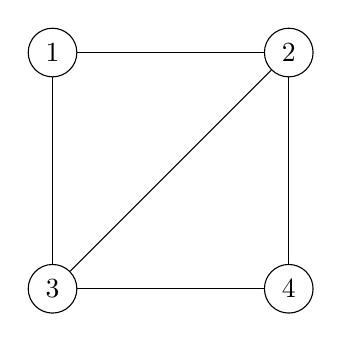
\begin{tikzpicture}[node distance={30mm}, main/.style = {draw, circle}] 
		\node[main] (1) {$1$}; 
		\node[main] (2) [right of=1] {$2$};
		\node[main] (3) [below of=1] {$3$};
		\node[main] (4) [below of=2] {$4$};
		\draw (1) -- (2);
		\draw (1) -- (3);
		\draw (2) -- (3);
		\draw (2) -- (4);
		\draw (3) -- (4);
	\end{tikzpicture}
	\caption{Primjer grafa s 4 vrha}
\end{figure}

Laplacian \textit{L} grafa sa slike 4.1 je:

\[
\centering
L = 
\begin{bmatrix}
	2 & -1 & -1 & 0 \\
	-1 & 3 & -1 & -1 \\
	-1 & -1 & 3 & -1 \\
	0 & -1 & -1 & 2
\end{bmatrix}
\]

Primjetimo da je suma svakog retka i stupca od \textit{L} jednak 0. Zbog toga je determinanta od \textit{L} uvijek jednaka 0.

Ako je $A$ s dimenzijama $n \times n$, s $A^{ij}$ se označava matrica dimenzija $(n - 1) \times (n - 1)$ dobivena brisanjem \textit{i}-tog redka i \textit{j}-tog stupca matrice \textit{A}. Takve matrice se nazivaju \textit{minore}. Sljedeći teorem nam govori da nam minore \textit{Laplaciana} grafa daju upravo rezultat koji tražimo.

\begin{theorem}[Matrični teorem o stablima]
Neka je G graf i neka T(G) označava broj razapinjućih stabala u G. Za bilo koji i, T(G) = $det L^{(ii)}$, gdje je L Laplacian od G. Determinanta $det L^{(ii)}$ ne ovisi o izboru parametra i.
\end{theorem}

\begin{proof}
Dokaz ćemo provesti matematičkom indukcijom. Pretpostavimo da teorem vrijedi za povezane grafove s manje vrhova ili bridova. Kao bazu indukcije, pretpostavimo da se graf \textit{G} sastoji od samo jednog vrha. U tom slučaju, $T(G) = 1$, i teorem daje ispravan rezultat: $L = [0]$ i $L^{(11)}$ po definiciji ima determinantu jednaku 1.

Ppretpostavimo sada da graf $G$ ima barem dva vrha, te označimo jedan od tih vrhova s $i$. Ako $i$ nije incidentan niti s jednim bridom, onda $G$ nema razapinjuće stablo jer nije povezan. U ovom slučaju će vrijediti tvrdnja teorema jer je $L^{(ii)}$ zapravo \textit{Laplacian} ostatka grafa te će njezina determinanta biti jednaka nuli.

\begin{figure}[htb]
	\minipage{0.33\textwidth}
	\begin{center}
		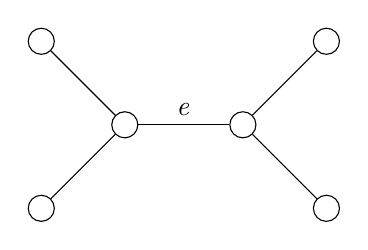
\begin{tikzpicture}[node distance={15mm}, main/.style = {draw, circle}] 
			\node[main] (1) {}; 
			\node[main] (2) [below right of=1] {};
			\node[main] (3) [right of=2] {};
			\node[main] (4) [above right of=3] {};
			\node[main] (5) [below left of=2] {};
			\node[main] (6) [below right of=3] {};
			\draw (1) -- (2);
			\draw (2) -- node[midway, above] {\textit{e}} (3);
			\draw (2) -- (5);
			\draw (3) -- (4);
			\draw (3) -- (6);
		\end{tikzpicture}
	\end{center}
	\caption*{\textit{G}}
	\endminipage\hfill
	\minipage{0.33\textwidth}
	\begin{center}
		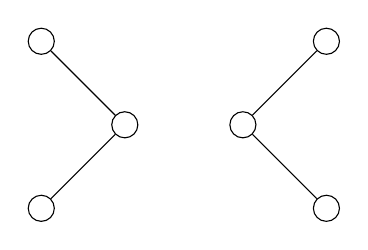
\begin{tikzpicture}[node distance={15mm}, main/.style = {draw, 	circle}] 
			\node[main] (1) {}; 
			\node[main] (2) [below right of=1] {};
			\node[main] (3) [right of=2] {};
			\node[main] (4) [above right of=3] {};
			\node[main] (5) [below left of=2] {};
			\node[main] (6) [below right of=3] {};
			\draw (1) -- (2);
			\draw (2) -- (5);
			\draw (3) -- (4);
			\draw (3) -- (6);
		\end{tikzpicture}
	\end{center}
	\caption*{\textit{G - e}}
	\endminipage\hfill
	\minipage{0.33\textwidth}
	\begin{center}
		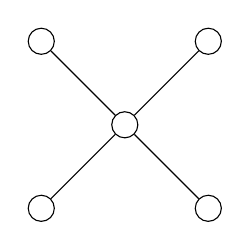
\begin{tikzpicture}[node distance={15mm}, main/.style = {draw, 	circle}] 
			\node[main] (1) {}; 
			\node[main] (2) [below right of=1] {};
			\node[main] (4) [above right of=2] {};
			\node[main] (5) [below left of=2] {};
			\node[main] (6) [below right of=2] {};
			\draw (1) -- (2);
			\draw (2) -- (5);
			\draw (2) -- (4);
			\draw (2) -- (6);
		\end{tikzpicture}
	\end{center}
	\caption*{$G \backslash e$}
	\endminipage\hfill
	\caption{$G - e$ je graf koji se dobije brisanjem brida \textit{e}, a $G \backslash e$ je graf koji se dobije kontrakcijom brida \textit{e} i spajanjem incidentnih vrhova u jedan vrh.}
\end{figure}

Sada pretpostavimo da je $i$ povezan s nekim drugim vrhom $j$, te neka $e$ označava brid $(i,j)$. Kao što je prikazano na slici 4.2, postoje dva načina na koje se može modificirati $G$: brid $e$ možemo jednostavno izbrisati, ili možemo kontrakcijom vrhove $i$ i $j$ spojiti u jedan vrh. Takve grafove označujemo s $G - e$ i $G \backslash e$. vrijedi da broj razapinjućih stabala $T(G)$ zadovoljava sljedeći rekurzivni izraz:

\begin{equation}
	T(G) = T(G - e) + T(G \backslash e)
\end{equation}

Ispravnost izraza (4.2) je dokazana u propoziciji 3.5.

Prema pretpostavci matematičke indukcije matrični teorem vrijedi za $G - e$ i za $G \backslash e$. Možemo razmjestiti vrhove od \textit{G} tako da su \textit{i} i \textit{j} prva dva vrha. Sada Laplacian \textit{L} od \textit{G} možemo napisati kao:

\[
L_G =
\begin{bmatrix}
	\begin{array}{c|c|c}
		d_i & -1 & r_i^T \\
		\hline
		-1 & d_j & r_j^T \\
		\hline
		r_i & r_j & L'
	\end{array}
\end{bmatrix}
\]

Ovdje $r^i$ i $r^j$ predstavljaju $(n - 2)$-dimenzionalne vektore koji opisuju povezanost vrhova $i$ i $j$ s ostalih $n - 2$ vrha od $G$ ($r_i^T$ i $r_j^T$ su transponirani vektori), a $L'$ je $(n - 2)$-dimenzionalna minora koja predstavlja \textit{Laplacian} ostatka grafa. Sada \textit{Laplaciane} grafova $G - e$ i $G \backslash e$ možemo zapisati na sljedeći način:

\[
L_{G - e} = 
\begin{bmatrix}
	\begin{array}{c|c|c}
		d_i - 1 & 0 & r_i^T \\
		\hline
		0 & d_j - 1 & r_j^T \\
		\hline
		r_i & r_j & L'
	\end{array}
\end{bmatrix},
L_{G \backslash e} = 
\begin{bmatrix}
	\begin{array}{c|c}
		d_i + d_j - 2 & r_i^T + r_j^T \\
		\hline
		r_i + r_j & L'
	\end{array}
\end{bmatrix}
\]

još je potrebno pokazati da vrijedi

\begin{equation}
	detL_G^{(ii)} = detL_{G - e}^{(ii)} + detL_{G \backslash e}^{(jj)},
\end{equation}

ili, u matričnom zapisu:

\[
det
\begin{pmatrix}
	\begin{array}{c|c}
		d_j & r_j^T \\
		\hline
		r_j & L'
	\end{array}
\end{pmatrix}
= det
\begin{pmatrix}
	\begin{array}{c|c}
		d_j - 1 & r_j^T \\
		\hline
		r_j & L'
	\end{array}
\end{pmatrix}
+ detL'.
\]

Ovaj rezultat slijedi iz činjenice da determinanta matrice može biti napisana kao linearna kombinacija njenih \textit{kofaktora}, tj. determinanti njenih minora. Za bilo koju matricu $A$ vrijedi

\begin{equation}
	detA = \sum_{j = 1}^{n} (-1)^j A_{1,j} detA^{(1,j)}.
\end{equation}

Dakle, ako se dvije matrice razlikuju samo u vrijednostima na poziciji (1,1) pri čemu je $a_{11} = b_{11} + 1$, a $A_{ij} = B_{ij}$ za svaki drugi $i$ i $j$, njihove determinante se razlikuju za determinantu njigovih (1,1) minora, odnosno $detA = detB + detA^{(1,1)}.$ Primjenimo li ovo za $L_G^{(ii)}$ i $L_{G - e}^{(ii)}$, dobit ćemo izraz (4.5), čime se dovršava dokaz ovog teorema.\footnote{Dokaz po uzoru na \cite{YWC}}
\end{proof}

\chapter{Prebrajanje razapinjućih stabala grafa pomoću matričnog teorema o stablima}

U ovom poglavlju primjenit ćemo matrični teorem o stablima za računanje broja razapinjućih stabala poznatih familija grafova. Za početak, za ilustraciju, evo jednog jednostavnog primjera.

\begin{figure}[htb]
	\centering
	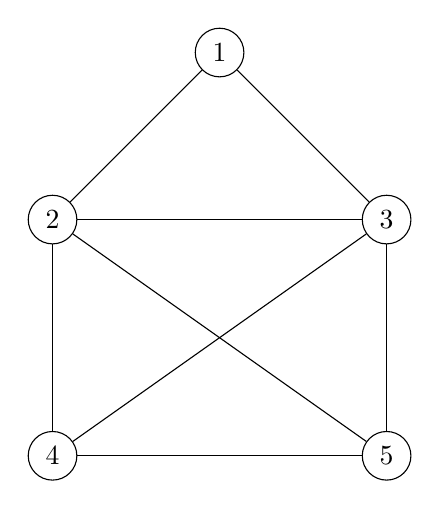
\begin{tikzpicture}[node distance={30mm}, main/.style = {draw, circle}] 
		\node[main] (1) {$1$}; 
		\node[main] (2) [below left of=1] {$2$};
		\node[main] (3) [below right of=1] {$3$};
		\node[main] (4) [below of=2] {$4$};
		\node[main] (5) [below of=3] {$5$};
		\draw (1) -- (2);
		\draw (1) -- (3);
		\draw (2) -- (3);
		\draw (2) -- (4);
		\draw (2) -- (5);
		\draw (3) -- (4);
		\draw (3) -- (5);
		\draw (4) -- (5);
	\end{tikzpicture}
	\caption{Primjer grafa s 5 vrhova}
\end{figure}

Na slici 5.1 prikazan je graf s 5 vrhova. Matrica susjedstva \textit{A} navedenog grafa, te njezin laplacian \textit{L} su sljedeći:

\[
\centering
A = 
\begin{bmatrix}
	0 & 1 & 1 & 0 & 0 \\
	1 & 0 & 1 & 1 & 1 \\
	1 & 1 & 0 & 1 & 1 \\
	0 & 1 & 1 & 0 & 1 \\
	0 & 1 & 1 & 1 & 0
\end{bmatrix}
, \quad
L = 
\begin{bmatrix}
	2 & -1 & -1 & 0 & 0 \\
	-1 & 4 & -1 & -1 & -1 \\
	-1 & -1 & 4 & -1 & -1 \\
	0 & -1 & -1 & 3 & -1 \\
	0 & -1 & -1 & -1 & 3
\end{bmatrix}
\]

Konstruirajmo zatim, na primjer, matricu \textit{L\textsuperscript{(22)}} dobivenu brisanjem drugog retka i drugog stupca matrice \textit{L}.

\[
\centering
L^{(22)} = 
\begin{bmatrix}
	2 & -1 & 0 & 0 \\
	-1 & 4 & -1 & -1 \\
	0 & -1 & 3 & -1 \\
	0 & -1 & -1 & 3
\end{bmatrix}
\]

Broj razapinjućih stabala grafa sa slike 5.1 jednak je determinanti prethodne matrice: $T(G) = det L^{(22)} = 40$. Jednak bi se rezultat dobio da smo matricu \textit{L\textsuperscript{(ii)}} stvorili tako da smo maknuli bilo koji drugi redak i stupac matrice \textit{L}.

Odredimo pomoću matričnog teorema o stablima eksplicitnu formulu za broj razapinjućih stabala potpunog grafa, $K_n$.

\begin{figure}[htb]
	\centering
	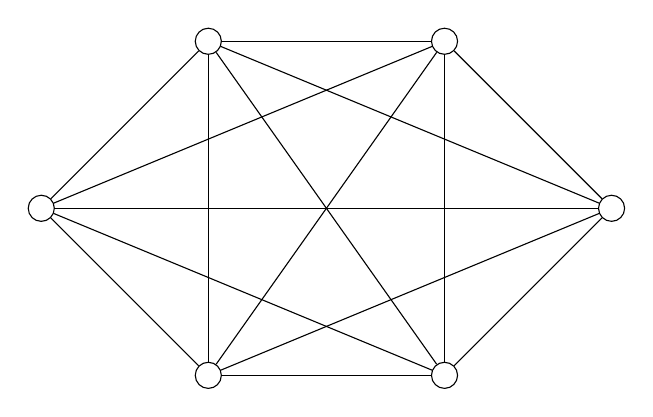
\begin{tikzpicture}[node distance={30mm}, main/.style = {draw, circle}] 
		\node[main] (1) {}; 
		\node[main] (2) [right of=1] {};
		\node[main] (3) [above right of=2] {};
		\node[main] (4) [above left of=3] {};
		\node[main] (5) [left of=4] {};
		\node[main] (6) [above left of=1] {};
		\draw (1) -- (2);
		\draw (1) -- (3);
		\draw (1) -- (4);
		\draw (1) -- (5);
		\draw (1) -- (6);
		\draw (2) -- (3);
		\draw (2) -- (4);
		\draw (2) -- (5);
		\draw (2) -- (6);
		\draw (3) -- (4);
		\draw (3) -- (5);
		\draw (3) -- (6);
		\draw (4) -- (5);
		\draw (4) -- (6);
		\draw (5) -- (6);
	\end{tikzpicture}
	\caption{Primjer potpunog grafa, $K_6$}
\end{figure}

Potpuni graf je graf u kojem je svaki vrh susjedan sa svim ostalim vrhovima. Primjer jednog potpunog grafa je dan na slici 5.2.

Poznato je da potpuni graf s $n$ vrhova, $K_n$, ima $n^{n-2}$ razapinjućih stabala. Sada ću taj rezultat dokazati pomoću matričnog teorema o stablima (za alternativni dokaz, vidi \cite{KKNP}).

Za potpuni graf $K_n$ s $n$ vrhova, pripadajuća matrica susjedstva je sljedeća:

\[
\centering
A = 
\begin{bmatrix}
	0 & 1 & 1 & \ldots & 1 & 1 \\
	1 & 0 & 1 & 1 & \ldots & 1 \\
	\vdots & \vdots & \ddots & & \ldots & \ldots  \\
	1 & 1 & \ldots & & 1 & 0
\end{bmatrix}
\]

Pripadni \textit{Laplacian} je:

\[
\centering
L = 
\begin{bmatrix}
	n-1 & -1 & -1 & \ldots & -1 & -1 \\
	-1 & n-1 & -1 & \ldots & \vdots & -1 \\
	\vdots & \vdots & \ddots & & \vdots & \vdots \\
	-1 & -1 & \ldots & & -1 & n-1
\end{bmatrix}
\]

Primjetimo da će minora te matrice, $L^{(ii)}$ biti ista bez obzira koji $i$ odabrali.

\[
\centering
L^{(ii)} = 
\begin{bmatrix}
	n-1 & -1 & -1 & \ldots & -1 & -1 \\
	-1 & n-1 & -1 & -1 & \vdots & -1 \\
	\vdots & \vdots & \ddots & & \vdots & \vdots  \\
	-1 & -1 & \ldots & & -1 & n-1
\end{bmatrix}
\]

Dimenzija prethodne matrice je $(n-1) \times (n-1)$. Sada je potrebno izračunati determinantu prethodne matrice. Počinjemo tako da prvom retku pribrojimo sve ostale retke. Dobit ćemo:
 
 \[
	\centering
	\left|
	\begin{matrix}
		1 & 1 & 1 & \ldots & 1 & 1 \\
		-1 & n-1 & -1 & -1 & \vdots & -1 \\
		\vdots & \vdots & \ddots & & \vdots & \vdots  \\
		-1 & -1 & \ldots & & -1 & n-1
	\end{matrix}
	\right|
\]
Sada ćemo prvi redak dodati svim ostalim retcima , te ćemo dobiti sljedeće:

 \[
\centering
\left|
\begin{matrix}
	1 & 1 & 1 & \ldots & 1 & 1 \\
	0 & n & 0 & 0 & \vdots & 0 \\
	\vdots & \vdots & \ddots & & \vdots & \vdots  \\
	0 & 0 & \ldots & & 0 & n
\end{matrix}
\right|
\]

Primjetimo da smo dobili gornju trokutastu matricu, a njena determinanta je jednaka umnošku elemenata na dijagonali, tako da je broj razapinjućih stabala potpunog grafa s $n$ vrhova, $T(K_n) = n^{n-2}$, što se poklapa s očekivanim rezultatom.

\chapter{Graphelite - računanje broja razapinjućih stabala}

\textit{\textbf{Graphelite}} je web-aplikacija koja korisniku omogućuje skiciranje jednostavnih grafova i izvršavanje raznih algoritama na zadanim grafovima. Omogućeno je crtanje grafova, određivanje minimalnog razapinjućeg stabla, određivanje duljine struka (najkraći ciklus), računanje kromatskog broja, bojanje vrhova grafa, te računanje broja razapinjućih stabala zadanog grafa.

\begin{figure}[htb]
	\centering
	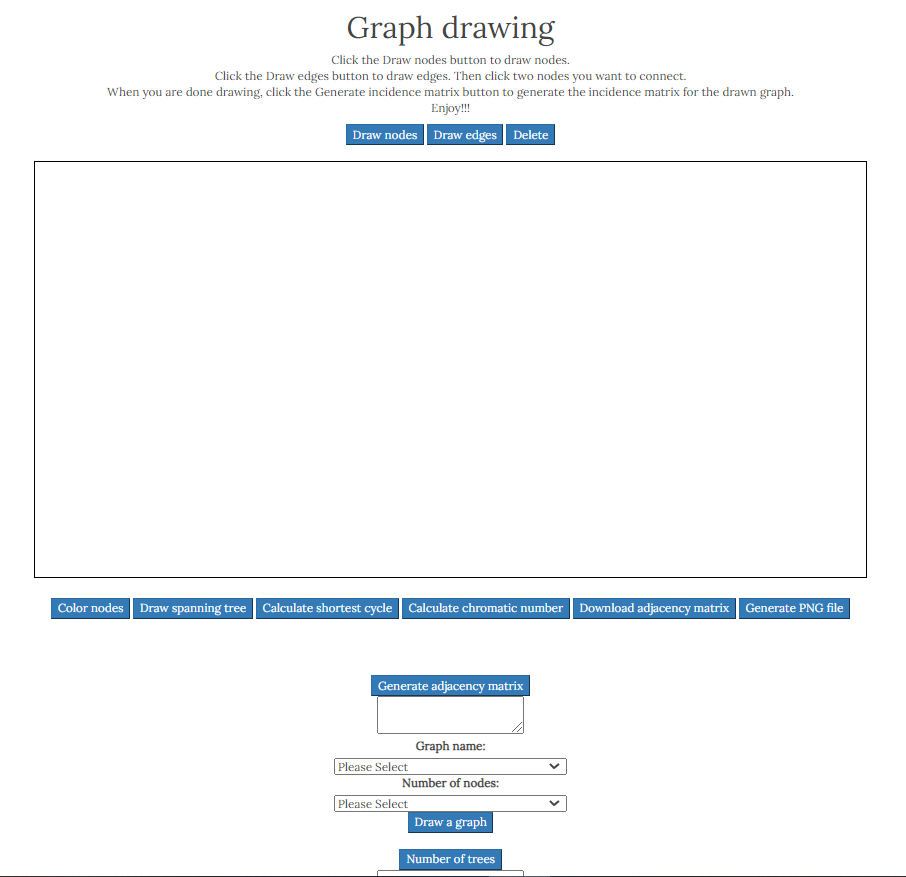
\includegraphics[width=0.5\textwidth]{slike/graphelite.png}
	\caption{Korisničko sučelje web-aplikacije \textit{Graphelite}}
	\label{fig:graphelite}
\end{figure}

\section{Računanje broja razapinjućih stabala grafa}

Broj razapinjućih stabala grafa kojeg korisnik grafički unese u aplikaciju se računa pomoću matričnog teorema o stablima koji je obrađen u 4. poglavlju ovoga rada. Odabere li korisnik opciju "Number of trees" pokrenut će se algoritam za izračunavanje broja razapinjućih stabala. Taj algoritam je sljedeći:

\begin{algorithm}
	\caption{Računanje broja razapinjućih stabala grafa}
	\label{algo:spanning-trees}
	\begin{algorithmic}
		\STATE{\textbf{Ulaz:} $matrix$ -- matrica susjedstva grafa $G$.}
		\STATE{\textbf{Ulaz:} $n$ -- broj vrhova grafa $G$}
		\STATE{\textbf{Izlaz:} broj razapinjućih stabala grafa $G$}
		\STATE{$L11 := array[n-1][n-1]$}
		\FOR{($i := 0; i < n - 1; i++$)}
			\FOR{($j := 0; j < n - 1; j++$)}
				\IF{$i == j$}
					\STATE{$num := 0$}
					\FOR{($k := 0; k < n; k++$)}
						\IF{$matrix[i+1][k] == 1$}
							\STATE{$num := num + 1$}
						\ENDIF
					\ENDFOR
					\STATE{$L11[i][j] := num$}
				\ELSIF{$matrix[i+1][j+1] == 1$}
					\STATE{$L11[i][j] := -1$}
				\ELSE
					\STATE{$L11[i][j] := 0$}
				\ENDIF
			\ENDFOR
		\ENDFOR
		\STATE{$rez := determinanta(L11)$}
		\RETURN{rez}
	\end{algorithmic}
\end{algorithm}

\newpage

\section{Demonstracija rada programa}

Prikazat ćemo rad algoritma za računanje broja razapinjućih stabala na primjerima Petersonovog grafa, i kotača sa 6 vrhova, \textit{W\textsubscript{6}}.

\subsection{Petersonov graf}

Na slici 6.1 se vidi Petersonov graf nacrtan u aplikaciji \textit{Graphelite}.

\begin{figure}[htb]
	\centering
	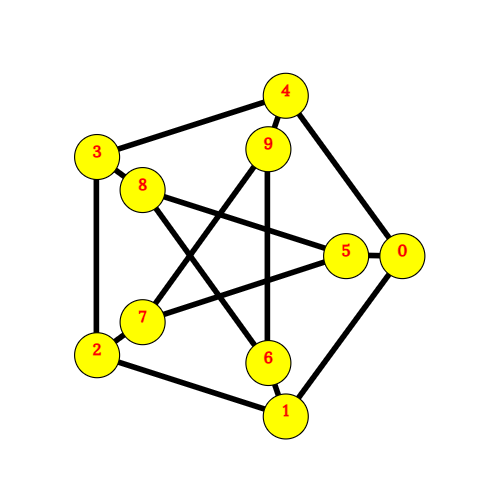
\includegraphics[width=0.5\textwidth]{slike/petersonov.png}
	\caption{Petersonov graf}
	\label{fig:petersonov}
\end{figure}

\begin{figure}[htb]
	\centering
	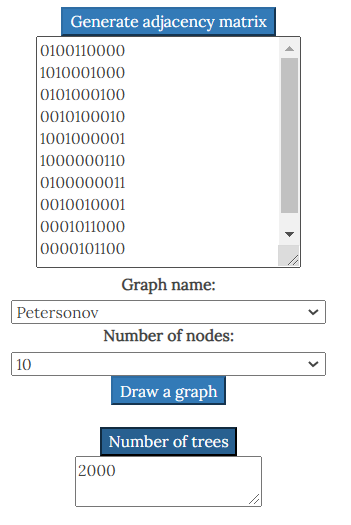
\includegraphics[width=0.5\textwidth]{slike/petersonovbroj.png}
	\caption{Broj razapinjućih stabala Petersonovog grafa}
	\label{fig:petersonov-broj}
\end{figure}

Na slici 6.2 vidi se matrica susjedstva Petersonovog grafa te broj razapinjućih stabala istog. Vidimo da je taj broj jednak 2000.

\subsection{Kotač sa 6 vrhova, \textit{W\textsubscript{5}}}

Na slici 6.3 se vidi graf kotač s 6 vrhova, \textit{W\textsubscript{5}} nacrtan u aplikaciji \textit{Graphelite}.

\begin{figure}[htb]
	\centering
	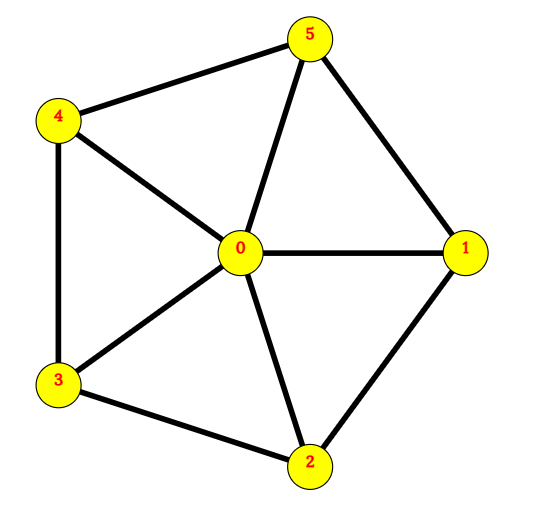
\includegraphics[width=0.5\textwidth]{slike/kotac2.png}
	\caption{Kotač $W_5$}
	\label{fig:kotac}
\end{figure}

\begin{figure}[htb]
	\centering
	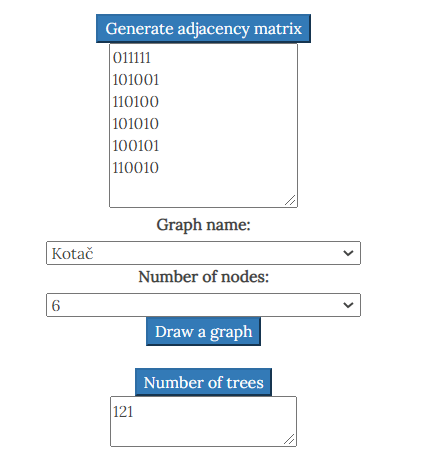
\includegraphics[width=0.5\textwidth]{slike/kotacbroj.png}
	\caption{Broj razapinjućih stabala grafa $W_5$}
	\label{fig:kotac-broj}
\end{figure}

Na slici 6.4 vidi se matrica susjedstva za \textit{W\textsubscript{5}} te broj razapinjućih stabala istog. Vidimo da je taj broj jednak 121, što smo i pokazali u ovom radu.

\chapter{Zaključak}


Upoznali smo se s pojmom grafa, iznijeli osnovne definicije i rezultate o grafovima. Nakon toga smo se upoznali s stablima, te pojmom razapinjućih stabala koji je i centralni pojam ovog rada.

U glavnom dijelu rada smo se bavili određivanjem broja razapinjućih stabala proizvoljnog grafa i utvrdili da ne postoji eksplicitna zatvorena formula. Dali smo primjer grafa kotača na kojem smo izračunali eksplicitnu formulu za određivanje broja razapinjućih stabala koristeći rekurzivne tehnike. Za poneke familije grafova je i moguće odrediti eksplicitnu formulu u ovisnosti o broju vrhova, no u općem slučaju, formula nije poznata.

Moćan alat za određivanje broja razapinjućih stabala grafa je opisan u radu. Teorem nam kaže da je broj razapinjućih stabala proizvoljnog grafa jednak determinanti proizvoljne minore \textit{Laplacove} matrice grafa $G$, koja se lako izvede iz matrice susjedstva od $G$.

To je elegantan rezultat koji možda čovjeku ne daje efikasan način ručnog računanja broja razapinjućih stabala (jer već i računanje determinante matrice koja ima dimenzije $8 \times 8$ može biti mukotrpan posao), ali omogućuje efektivno računalno rješavanje problema pri čemu je brzina rješavanja problema jednaka brzini računanja determinante. 

Predstavljena je i web-aplikacija \textit{Graphelite} koja korisniku omogućuje crtanje grafova i provedbu raznih korisnih algoritama. Među njima je i algoritam za računanje broja razapinjućih stabala, i njegov pseudokod je napisan u ovom radu.

\bibliographystyle{fer}

\begin{thebibliography}{6}
	\bibitem{MM}
	C. Moore, S. Mertens, The Nature of Computation, Oxford University Press Inc., New York, 2011.
	\bibitem{MB}
	M. Bóna, A Walk Through Combinatorics: An Introduction to Enumeration and Graph Theory, 4. izdanje, World Scientific, New Yersey, 2017.
	\bibitem{KKNP}
	D. Kovačević, M. Krnić, A. Nakić, M.O. Pavčević, Diskretna matematika 1, FER, Zagreb, rujan 2019.
	\bibitem{YWC}
	B. Ye Wu, K. Chao, Spanning Trees and Optimization Problems, Chapman \& Hall/CRC, 2004.
	\bibitem{SND}
	S.N. Daoud, Complexity of graphs generated by wheel graph and their asymptotic limits, Journal of the Egyptian Mathematical Society 25, 2017., 424--433
	\bibitem{NE}
	N. Elezović, Linearna algebra, Element, Zagreb, 2016.
\end{thebibliography}

\begin{sazetak}
Tema ovog rada je prebrojavanje razapinjućih stabala grafa. Predstavljeni su osnovni pojmovi teorije grafova, zatim je predstavljen pojam razapinjućeg grafa, razne primjene, te računanje broja razapinjućih stabala pomoću rekurzivnih relacija. Predstavljeni su iskaz i dokaz matričnog teorema o stablima, te primjene. Na kraju je prikazan rad web-aplikacije \textit{Graphelite} za računanje s grafovima.

\kljucnerijeci{teorija grafova, stabla, razapinjuća stabla, matrični teorem o stablima}
\end{sazetak}

\engtitle{Counting spanning trees of a graph}
\begin{abstract}
The thesis for this paper is counting spanning trees. I presented the basic concepts of graph theory, then I introduced the spanning trees and connected them with some applications. I expressed and proved the Matrix-tree theorem and connected it with applications. In the end, I showed the implementation of the \textit{Graphelite} web-application for working with graph theory.

\keywords{graph theory, trees, spanning trees, matrix-tree theorem}
\end{abstract}

\end{document}
